\section{Igor Wadas}
\label{sec:iwadas}

\subsection{Zdjecie}
Losowe zdjecie(see Figure~\ref{fig:carti})


\begin{figure}[htbp]
    \centering
    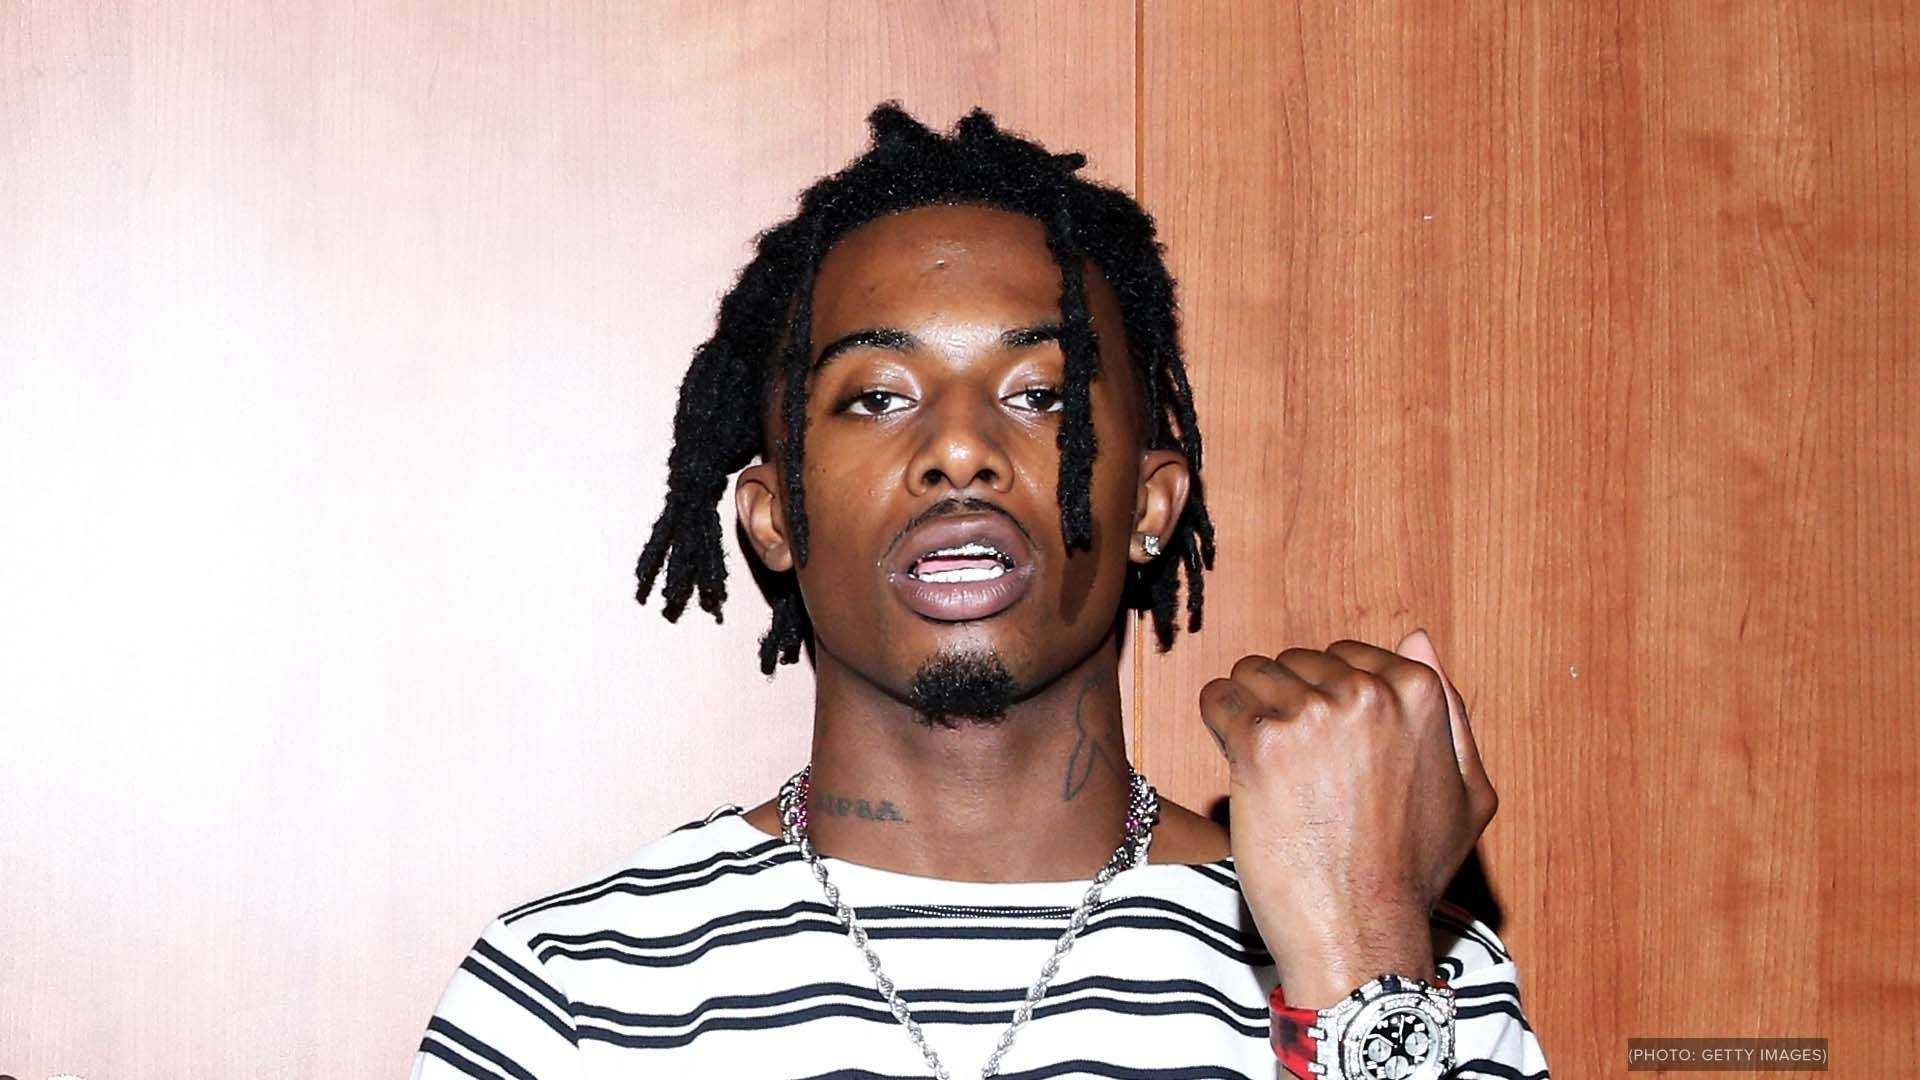
\includegraphics[width=0.6\textwidth]{pictures/IgorWadas.jpg}
    \caption{Playboi Carti}
    \label{fig:carti}
\end{figure}

\subsection{Tablica}
Sudoku to logiczna lamiglowka, w ktorej celem jest wypelnienie planszy 9x9 liczbami od 1 do 9 w taki sposob, aby kazda kolumna, kazdy wiersz i kazdy z dziewieciu 3x3 obszarow nie zawieral powtarzajacych sie cyfr. Table~\ref{tab:sudoku} pokazuje przykladowa plansze do sudoku.
\begin{table}[htbp]
\centering
\begin{tabular}{||l|l|l||l|l|l||l|l|l||} \hline\hline
  &   &   & 8 &   &   &   &   & 9 \\\hline
  & 1 & 9 &   &   & 5 & 8 & 3 &   \\\hline
  & 4 & 3 &   & 1 &   &   &   & 7 \\\hline\hline
4 &   &   & 1 & 5 &   &   &   & 3 \\\hline
  &   & 2 & 7 &   & 4 &   & 1 &   \\\hline
  & 8 &   &   & 9 &   & 6 &   &   \\\hline\hline
  & 7 &   &   &   & 6 & 3 &   &   \\\hline
  & 3 &   &   & 7 &   &   & 8 &   \\\hline
9 &   &   & 5 &   &   &   &   & 1 \\ \hline\hline
\end{tabular}
\label{tab:sudoku}
\caption{Plansza sudoku}
\end{table}

\subsection{Wyrazenie matematyczne}
Rownania matematyczne
$$ e^{i\pi} + 1 = 0$$
$$\lim_{x \to 2} \frac{x^2 - 4}{x - 2} = 4$$

\subsection{Tablica nienumerowana}
\begin{itemize}
  \item jeden
  \item dwa
  \item trzy
\end{itemize}

\subsection{Tablica numerowana}

\begin{enumerate}
\item pencil 
\item ruler
\item notebook
    \begin{enumerate}
    \item pencil 
    \item ruler
    \begin{enumerate}
        \item something
        \item something
        \item something
        \item something
        \item something
        \item something
        \item something
        \item something
        \item something
    \end{enumerate}
    \item notebook
    \item calculator
    \end{enumerate}
\item calculators
\end{enumerate}

\subsection{Tekst z akapitami}
\begin{center}

To jest przykład tekstu w \LaTeX.
\begin{flushleft}
    Oto akapit, który zawiera zarówno
\textbf{tekst zgrubiony}, jak i \textit{tekst w kursywie}.\end{flushleft}
\par Możesz dowolnie formatować tekst w \LaTeX, aby spełnić swoje potrzeby.

\end{center}